\section{Mathematical Optimization}

\todo{meaning of program}
% Mathematical optimization or mathematical programming .... The term "programming" does not come from computer programs but dates back to the 1940s and ...

An optimization problem is defined as:
\begin{mini!}
    {\scriptstyle \bold x \in \mathbb{R}^n}{f(\bold x)}{ \label[problem]{problem:optimization_problem}}{}
    \addConstraint{g_i(\bold x) \leq 0, \quad i=1,...,m} 
\end{mini!}

where \todo{put comma ?} $f$ is the \textit{objective function}, $g_i$ are the \textit{constraint functions} and $\bold x$ are the \textit{decision variables}. \cite{boyd_stephen_convex_2004}
The \textit{feasible region} is the set of all points that respect the constraints. An optimization problem with a constrained feasible region is often also called \textit{constrained optimization problem} in contrast to an \textit{unconstrained optimization problem}. A \textit{solution} is a vector $\bold x$ that lies in the feasible region. An \textit{optimal solution} $\bold x^*$ is a solution with the smallest objective value. The \textit{objective value} of $\bold x^*$ is the value of the objective function evaluated at $\bold x^*$. If a problem has no solution it is said to be \textit{infeasible}. A problem is \textit{unbounded} if solutions exist, but the objective value can be arbitrarily small.
One can maximize over a function $f$ by setting the objective function to $\min -f(\bold x)$.
Depending on the type of the objective function and the type of constraints, optimization problems are divided into different classes of optimization problems. The classes relevant for this thesis are linear programs, mixed-integer programs and disjunctive programs. 
Different algorithms can be used depending on the problem structure.
\unsure[inline]{type of ll FBA problem, write about bilinear constraints ??}
% \todo{or define solution as optimal solution}

\subsection{Preliminaries and Notation}
\todo[inline]{update vector, matrix notation in thesis, use variables consistently, check when to use if and when iff, which words to write in italic}

\begin{enumerate}
    \item The set $\mathbb{R}$ denotes the set of real numbers and the set $\mathbb{Z}$ denotes the set of whole numbers. If scalar $\alpha$ is in the set of real numbers, we write $\alpha \in \mathbb R$. %(instead of $\mathbb R ^1$)
    
    \item A vector $\bold{v} = (v_1, ..., v_n) \in \mathbb{R}^n$ is identified as column vector and printed in bold. $\bold v \tran$ transposes $\bold v$ into a row vector. The inner product of two vectors $v, w \in \mathbb{R}^n$ is $\bold v \tran \bold w = \sum_{i=1}^n v_i w_i$. $\bold v \leq \bold w$ denotes element-wise inequality. $\log (\bold v)$ denotes the element-wise logarithm. The 1-vector is written as $\bold 1 := (1, 1, ..., 1) \in \mathbb{R}^n$ the 0-vector as $\bold 0 := (0, 0, ..., 0) \in \mathbb{R}^n$. The \textit{support} of $\bold{v}$ is the set of indices $i$ with $v_i \neq 0$ and is denoted by $\text{supp}(\bold v)$.

    \item The entry in row $i$ and column $j$ of a matrix $ \bold A \in \mathbb{R}^{n \times m}$ is denoted as $a_{i,j}$. The $i$-th row is $\bold a_{i,*}$ and the $j$-th column $\bold a_{*,j}$. \todo{update in entire section, often one index used for row of matrix}
    
    \item Let $\bold A \in \mathbb{R}^{n \times n}$ be an invertible matrix: $ \bold A \bold A^{-1} = \bold I$, where $\bold I$ is the identity matrix. The matrix $ \bold A^{-1}$ is the inverse matrix of $ \bold A$. \todo{when is matrix invertible}

    \item A \textit{linear combination} is defined as $\sum_{i=1}^{m} \lambda_i \bold x_i = 
    \lambda_i \bold x_1 + ... + \lambda_m \bold x_m$, where $\lambda_i \in \mathbb{R}$ and $\bold x_i \in \mathbb{R}^n$.
    A line going through point $\bold x$ generated by $\bold r \in \mathbb{R}^n$ is the set $\{\bold x + \lambda \bold r | \lambda \in \mathbb{R}\}$. A \textit{line segment} is a subset of a line defined on the interval between $l \in \mathbb{R}$ and $u \in \mathbb{R}$: $\{\bold x + \lambda \bold r | \lambda \in \mathbb{R}, \, \lambda \in [l, u ]\}$.

    \item A \textit{Basis} $B$ of vector space $V$ is a set of vectors $(\bold v_1, \bold v_2, ..., \bold v_n)$ that are linearly independent and every $\bold v \in V$ can be written as a linear combination of vectors in $B$.

    \item The \textit{nullspace} of matrix $\bold A \in \mathbb{R}^{n \times m}$ is defined as $\text{null}(\bold A):=\{\bold x \in \mathbb{R}^n: \bold A \bold x = \bold 0\}$. \todo{rowspace} 
    
    \item A set $C \subseteq \mathbb{R}^n$ is \textit{convex} if for any two points $\bold x, \bold y \in C$ the line segment between them is in $C$. %every convex combination for any two points $x,y \in X$ is contained in $C$.
    The \textit{convex hull} of a set $X$ is the smallest convex set that contains all points in $X$ and denoted as $\text{conv}(X)$. It is a set of convex combinations such that all points $x_i$ in $X$ can be represented, where a \textit{convex combination} is a linear combination with $\lambda_i \geq 0$ and $\sum_{i=1}^m \lambda_i = 1$.
    
    \item The set $\{x \in \mathbb{R}^n | \alpha \tran x = \beta \}$ is a \textit{hyperplane}, where $\alpha \in \mathbb{R}^n$ and $\beta \in \mathbb{R}$. The set $\{x \in \mathbb{R}^n | \alpha \tran x \leq \beta \}$ is a \textit{half-space}. \cite{understanding_lp}
    A \textit{polyhedron} is the intersection of a finite number of half-spaces: $P = \{ \bold x | \bold Ax \leq \bold b\}$. Hyperplanes, half-spaces and polyhedra are convex. A point $x \in P$ is an \textit{extreme point} or \textit{vertex} if it cannot be represented as a convex combination of any other points in $P$. %\todo{closed halfspace needed?}
   
    \item A set $C \subseteq \mathbb{R}^n$ is a \textit{cone} if $\lambda x \in C$ for any $x \in C$ and $\lambda \geq 0$. A \textit{conic combination} is a linear combination with $\lambda \geq 0$. A cone is a \textit{convex cone} if it contains the conic combinations of all $x_i \in C$. $C$ is \textit{pointed} if it contains no line and the extreme point is called $apex$. A vector $r \in \mathbb{R}^n$ is a \textit{ray} of $C$ iff $\{x_i + \lambda r | \lambda \geq 0 \} \in C$ for any $x_i \in C$ and non-zero $r$. Ray $r$ is an \textit{extreme ray} if it cannot be represented by a conic combination of other rays in $C$. 
    A cone is $polyhedral$ if the number of extreme rays is finite. A cone is \textit{simplicial} if it has $n$ extreme rays. \todo{verify}
    The \textit{conic relaxation} of an extreme point $x$ of a polytope $P$ is a cone with apex $x$ and where the extreme rays are the half-spaces of $P$ intersecting at $x$.
    
    % \unsure[inline]{how to define ray, as r as lambda r or as x + lambda r}

    \item A set $S$ is \textit{closed} if the limit points of a set are all contained in the set. The limit points of a set are the limits of sequences of elements of that set. The \textit{interior} of a set $S$ is denoted by $\text{int}(S)$.
\end{enumerate}
\todo[inline]{remove polytope from examples}
\todo[inline]{align all problems that are on the same page} 
\todo{use Problem instead of Equation}

\subsection{Linear Programming} \label{Section:Linear Programming}
A \textit{linear program} (LP) is an optimization problem with a linear objective function and linear constraints.

\begin{mini!}
    {\scriptstyle x}{\bold c\tran \bold x}{\text{\textbf{LP:}} \label[problem]{problem:LP}}{}
    \addConstraint{\bold A \bold x\leq \bold b} 
    \addConstraint{\bold x \in \mathbb{R}^n}
    % \addConstraint{x\geq \bold 0} 
\end{mini!}

where $\bold c \in \mathbb{R}^n$, $ \bold A \in \mathbb{R}^{m \times n}$ \todo{x positive ?} and $\bold b \in \mathbb{R}^m$. It is assumed that the number of constraints $m$ is greater than the number of variables $n$, to have an \textit{underdetermined} system of linear equations which allows to have many solutions. \todo{should it be $\leq$ ?} The linear inequalities define a convex polyhedron. If an optimal solution exists, there exists an optimal solution at one of the vertices. In that case, the LP can have exactly one optimal solution, or multiple optimal solutions if an entire edge or face is optimal. An LP has no optimal solution if it is infeasible or unbounded.

We want to solve the following optimization problem:
\begin{equation} \label[problem]{problem:lp_example}
    \text{max} \{y \, : \, 0 \leq x \leq 3 , \, 0.5 \leq y \leq 4, \, y \leq 1.5 x + 0.5, \, y \leq -0.5 x + 4.5, \, x,y \in \mathbb{R} \}
\end{equation} 
There are two decision variables $x, y$. We want to find a solution $(x^*, y^*)$ with maximal $y$-value such that the constraints are respected. The problem is a linear program and can be written as \cref{problem:LP} by simple linear transformations. If we want to write \cref{problem:lp_example} as a minimization problem, the objective becomes $-y$. If we visualise the example (\cref{fig:lp}), we see that there exists one optimal solution located at $(2,3.5)$. Usually we are interested in problems in higher dimensions and it is not possible to solve them visually.
\todo{why orthogonal line to objective function has the same objective values}

\begin{figure}[h!]
    \caption{visualization of \cref{problem:lp_example}}
    \centering
    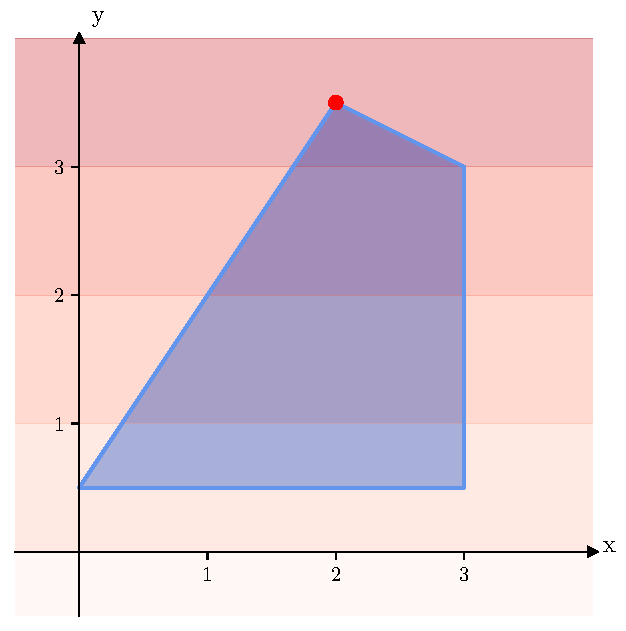
\includegraphics[width=0.6\textwidth]{Images/lp.pdf}
    \label{fig:lp}
    \subcaption{
        The set of feasible solutions contains all the points in the interior or on the boundary of the polytope (blue line segments). The optimal solution $x^*$ is the point in the feasible region with the biggest $y$-value (red point). The isolines indicate the function value of the points.}
\end{figure}

An LP is said to be in \textit{standard form} if it is of the form:
\begin{mini!}
    {\scriptstyle x}{\bold c\tran \bold x}{\label[problem]{problem:LP_standard_form}}{}
    \addConstraint{\bold A \bold x = \bold b} 
    \addConstraint{\bold x \geq \bold 0} 
\end{mini!}

where $\bold c, \bold x \in \mathbb{R}^n, \, \bold A \in \mathbb{R}^{m \times n}$ and $\bold b \in \mathbb{R}^m$. Any LP can be written in standard form by adding one \textit{slack variable} per inequality to write it as equality. $\bold a_{i,*} \tran \bold x \leq b_i$ becomes $\bold a_{i,*} \,\tran \bold x + s_i = b_i$ with $s_i \geq 0$.\todo{split x into nonpositive and nonnegative parts}
\cite{noauthor_numerical_2006}

A vertex of the feasible region is also called \textit{basic feasible solution}. Suppose we have an LP in polyhedral form as in \cref{problem:LP}. Let $\bold x \in \mathbb{R}^n$ be a basic feasible solution. There exist $n$ constraints that are a basis of $\bold x$. $B$ is the set of constraint indices that are in the basis. Any variable $x_i \in B$ is a \textit{basic variable}. A variable $x_i \not \in B$ is a \textit{nonbasic variable} and $x_i=0$ \cite{understanding_lp}.

\subsubsection{Solving LPs}
There exist several algorithms that solve linear programs. The \textit{ellipsoid method} is the first algorithm that was proven to have a polynomial runtime in the worst case. However, in practise other algorithms outperform it. Another class of algorithms are \textit{interior point methods}. Some interior point methods have a polynomial runtime in the worst case and are used in practise. Interior point methods start with a feasible solution in the interior of the feasible region and approach the optimum without stepping outside of the feasible region. \cite{understanding_lp}

Another algorithm that is relevant in practise is the \textit{simplex algorithm}. It is based on the fundamental property of LPs that the optimum is located at one of the vertices of the feasible region. In \textit{phase \RomanNumeralCaps{1}} of the algorithm a vertex of the feasible region is computed. In \textit{phase \RomanNumeralCaps{2}} the algorithm moves from vertex to vertex along edges of the feasible region. The \textit{pivot rule} determines to which vertex to move next. There exist several pivot rules, however for all of them, there are families of problem instances on which the number of pivot steps needed grows exponentially. The worst case runtime on some instances is in conflict with the observed polynomial runtime in practise. Studying the simplex method with \textit{smoothed analysis} which tries to close this gap and shows a polynomial runtime of the simplex method. In smooth analysis a small noise is added to the entries of a fixed instance and afterwards worst-case analysis is performed on the perturbed instance \cite{huiberts}, \cite{dadush}.
% \todo[inline]{when which algorithm is better}

\subsubsection{Optimality and Duality}
An optimization problem can be written as an unconstrained problem by augmenting the objective function with a weighted sum of the constraints. The resulting function is known as the \textit{Lagrangian}.
The Lagrangian of an LP in standard form is: 
\begin{equation} \label{Eq:lagrangian}
\mathcal{L} (\bold x, \boldsymbol{\lambda}, \boldsymbol \nu) = \bold c \tran \bold x - \sum_{i=1}^n \lambda_i (x_i) - \sum_{i=1}^m \bold \nu_i (A_{i,*} \tran \bold x - b_i)
\end{equation} \todo{$\lambda_i (x_i)$ correct?}
where $\lambda_i \geq 0$ and $\nu_i \in \mathbb{R}$ are called \textit{Lagrange multipliers} or \textit{dual variables}.
For unconstrained problems with a differentiable and convex objective function, the KKT-conditions are a proof for optimality of a solution. As the objective function in linear programs is convex, we obtain the optimality conditions captured in \cref{theorem:lp_duality}. \cite{boyd_stephen_convex_2004} 

\begin{theorem}[Optimality conditions for LPs] \label{theorem:lp_duality}
    A solution $\bold x^*$ is optimal if there exist vectors $\boldsymbol \lambda$ and $\boldsymbol \nu$ that satisfy the following conditions \cite{noauthor_numerical_2006}:
    \begin{enumerate}
        \item $\boldsymbol \lambda + \bold A \tran \boldsymbol \nu = \bold c $
        \item $ \bold A \bold x - \bold b = \bold 0$
        \item $\bold x \geq \bold 0$
        \item $\boldsymbol \lambda \geq \bold 0$
        \item $\bold x \tran \boldsymbol \lambda = \bold 0$
    \end{enumerate}
\end{theorem} 
\todo{cite: following mostly taken from \cite{aps_mosek_nodate}}
We call a linear program in standard form as in \cref{problem:LP_standard_form} the \textit{primal problem}.
The associated \textit{dual function} of the primal problem is: 
\begin{align*}
    q(\boldsymbol \lambda, \boldsymbol \nu)
    & = \min_{\bold x} \mathcal{L} (\bold x, \boldsymbol \lambda, \boldsymbol \nu) \\
    & = \min_{\bold x} \bold c \tran \bold x - \boldsymbol \lambda \tran \bold x - \boldsymbol \nu \tran (A \bold x - \bold b) & \\
    & = \min_{\bold x} \bold c \tran \bold x - \boldsymbol \lambda \tran \bold x - \boldsymbol \nu \tran A \bold x + \boldsymbol \nu \tran \bold b  &\\
    & = \min_{\bold x} (\bold c \tran - \boldsymbol \lambda \tran - \boldsymbol \nu \tran A) \bold x + \boldsymbol \nu \tran \bold b  &\\
    & = \min_{\bold x} \bold x \tran (\bold c - \boldsymbol \lambda - A \tran \boldsymbol \nu) + \bold b \tran \boldsymbol \nu &\\
    & = \left\{
    \begin{array}{lr}
        \bold b \tran \boldsymbol \nu \quad \quad \text{if} \, \, \bold c - \boldsymbol \lambda - A \tran \boldsymbol \nu = \bold 0\\
        - \infty \quad \quad \text{otherwise}
    \end{array}
\end{align*}
Given a feasible solution $\bold x'$ \todo{do not use '} for the primal problem and a feasible solution $(\boldsymbol \lambda ', \, \boldsymbol \nu ')$ for the dual problem. If the dual function is bounded we know that $\bold c - \boldsymbol \lambda' = A \tran \boldsymbol \nu'$ and we know that $\bold x'$ satisfies $ \bold A\bold x' = \bold b$. The function value $q(\boldsymbol \lambda', \boldsymbol \nu')$ is a lower bound on the objective value of the primal problem: 
\begin{equation*}
    \bold b \tran \boldsymbol \nu' 
    = (A \bold x') \tran \boldsymbol \nu' 
    = \bold x' \tran A \tran \boldsymbol \nu' 
    = \bold x' \tran (\bold c - \boldsymbol \lambda') 
    = \bold c \tran \bold x'  - \boldsymbol \lambda' \tran \bold x'
    \leq \bold c \tran \bold x'
\end{equation*}
The tightest bound maximizes $\bold b \tran \boldsymbol \nu$. Formulated as a linear program we obtain the \textit{dual problem}:
\begin{maxi!}
    {\scriptstyle \boldsymbol \nu, \boldsymbol \lambda}{\bold b \tran \boldsymbol \nu}{\label[problem]{problem:dual_problem_slack}}{}
    \addConstraint{\boldsymbol \lambda + \bold A \tran \boldsymbol \nu = \bold c} 
    \addConstraint{\boldsymbol \lambda \geq \bold 0} 
\end{maxi!}
or rewritten without the slack variables $\boldsymbol \lambda$:
\begin{maxi!}
    {\scriptstyle \boldsymbol \nu}{\bold b \tran \boldsymbol \nu}{\label[problem]{problem:dual_problem}}{}
    \addConstraint{\boldsymbol A \tran \boldsymbol \nu \leq \bold c} 
\end{maxi!}
\todo[inline]{add dimensions to all variables, mention other shapes of primal}

Let $p^*$ be the objective value of an optimal solution for the primal problem and $d^*$ the objective value of an optimal solution to the dual problem. We have seen that $d^*$ is a lower bound on $p^*$ which is known as \textit{weak duality}. 
\begin{theorem}[Strong Duality] \label{theorem:strong_duality}
    Given a primal (P) and corresponding dual program (D), exactly one of the following is true \cite{noauthor_numerical_2006}:
    \begin{enumerate}
        \item P and D both have at least one optimal solution with objective values $p^*$ and $d^*$ and  $p^*=d^*$
        \item either P or D is unbounded and the other is infeasible
    \end{enumerate}
\end{theorem}
For linear programs \textit{strong duality} holds. A proof for \cref{theorem:strong_duality} can be found in \cite{aps_mosek_nodate}. Property (1) of \cref{theorem:strong_duality} is used to prove optimality of a solution. 

% \todo[inline]{example + visualization}
% \begin{lemma}[Farkas Lemma]
%     Given an LP in standard form, exactly one of the following is true:
%     \begin{enumerate}
%         \item the LP has at least one solution $x$
%         \item there exists a vector $y$ such that $ \bold A \tran y \leq 0$ and $b \tran y > 0$
%     \end{enumerate}
% \end{lemma}

% \cite{aps_mosek_nodate}

\subsection{Mixed-Integer Programming} \label{Section:MIP}
Many problems in practise cannot be formulated by only using linear constraints and continuous decision variables. It is often required that a subset of variables is discrete. A \textit{mixed-integer program} (MIP) is an optimization problem with a linear objective function, linear constraints and a subset of integer variables:

\begin{mini!}
    {\scriptstyle x}{\bold c\tran \bold x}{\text{\textbf{MIP:}} \label[problem]{problem:MIP}}{}
    \addConstraint{\bold A \bold x\leq \bold b} 
    % \addConstraint{x\geq \bold 0} 
    \addConstraint{\bold x \in \mathbb{Z}^{|J|} \times \mathbb{R}^{n-|J|}}
\end{mini!}

where $\bold c \in \mathbb{R}^n, \, \bold A \in \mathbb{R}^{m \times n}$, $\bold b \in \mathbb{R}^m$. The set $J$ contains the indices of integer variables. 

Let us reuse the LP example in \cref{Section:Linear Programming} and add integrality constraints on the decision variables $x$ and $y$:
\begin{equation} \label[problem]{problem:mip_example}
    \text{max} \{y \, : \, 0 \leq x \leq 3 , \, 0.5 \leq y \leq 4, \, y \leq 1.5 x + 0.5, \, y \leq -0.5 x + 4.5, \, x,y \in \mathbb{Z} \}
\end{equation} 

Looking at the visualisation of the problem (\cref{fig:mip}), we see that the optimal solution of the LP $x^{LP} = (2,3.5)$ is no valid solution for the MIP formulation. The points $(2,3)$ and $(3,3)$ are the optimal solutions.

\begin{figure}[h!]
    \caption{visualisation of \cref{problem:mip_example}}
    \centering
    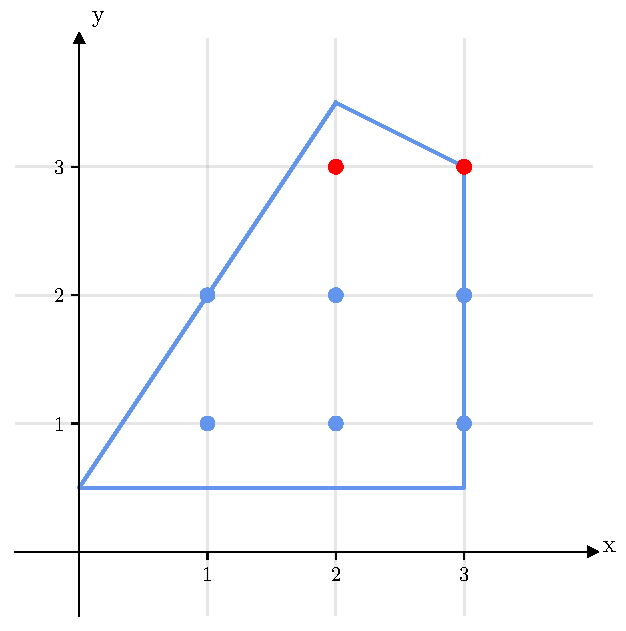
\includegraphics[width=0.6\textwidth]{Images/mip.pdf}
    \label{fig:mip}
    \subcaption{
        The feasible points of the MIP are the integer points respecting the polyhedral constraints (blue points). The set of feasible solutions to the relaxed LP is are all the points in the interior or on the boundary of the polytope (blue line segments). An optimal solution is a point in the feasible region with the biggest $y$-value (red point). The optimal solutions are at $(2,3)$ and $(3,3)$.}
\end{figure}

The MIP formulation enables us to model much more complex problems. Apart from incorporating discrete quantities, it is possible to capture Boolean expressions. Suppose we want to model the \textit{indicator constraint} $z = 1 \implies \bold a \tran \bold x \leq b$. We can reformulate the constraint with a linear constraint using the \textit{big-M method}: 
\begin{equation*}
    \bold a \tran \bold x \leq b + M(1-z)
\end{equation*}
If $z=1$ the constraint is enforced. In the case $z=0$, the value of $M$ has to be larger than $\bold a \tran \bold x - b$ such that the constraint is inactive \cite{aps_mosek_nodate}.

\subsubsection{Solving MIPs}
Solving MIPs is much more complicated than solving LPs, because it is not guaranteed that if an optimal solution it is at one of the vertices. In general, solving MIPs is $\mathcal{NP}$-hard. \todo{formulated as decision problem NP-complete; solution verifiable in polynomial time} Instead of solving the MIP directly, a sequence of \textit{LP relaxations} is solved: the integrality constraints are ignored and the constraint in \cref{problem:MIP} (c) becomes $\bold x \in \mathbb{R}^n$.

Let $z^{LP}$ be the objective value of an optimal solution $\bold{x}^{LP}$ of the LP relaxation and $z^*$ the objective value of an optimal solution $\bold{x^*}$ to the MIP problem. We know that: 
\begin{equation*} \label{Eq:bound}
    z^{LP} \leq z^*
\end{equation*}
One common approach for solving MIPs is the \textit{branch-and-bound} algorithm. The idea is to generate a branch-and-bound tree starting with the solution to the LP relaxation $\bold x^{LP} \in \mathbb{R}^n$ at the root node. A variable $x_i$ that should be integer according to the MIP formulation that is fractional in $\bold x^{LP}$ is selected as \textit{branching variable}. We divide the search space $P$ by creating two child nodes. In one $x_i$ has to be larger or equal to the rounded up value and the feasible region becomes $P \cap \{x_i \geq \lceil x_i^{LP} \rceil \}$. In the other child node, $x_i$ can take at most the rounded down value of $x_i^{LP}$ and the feasible region of the subproblem is $P \cap \{x_i \leq \lfloor x_i^{LP} \rfloor \}$\todo{correct?}. The solution with the smallest objective value respecting the MIP formulation is called \textit{incumbent} and the objective value is denoted by $z^{INC}$. We continue branching until all variables in $J$ are integral, a subproblem is infeasible or if a node can be $pruned$. The optimal solution in each node $i$ is bounded by the objective value of the relaxed solution $z^{LP}_{(i)}$. If $z^{LP}_{(i)}$ is greater or equal to $z^{INC}$, node $i$ is cut off the tree. 

% \todo{add figure for branching}

Another approach is the \textit{cutting plane} algorithm. The LP relaxation can be very weak. As we are dealing with a linear objective, we could get the optimal MIP solution easily if we had access to the \textit{integer hull}: $\text{conv}(P \cap \mathbb{Z}^n)$. As this is usually not the case, one can tighten the LP relaxation by adding \textit{cuts}. A cut is an inequality that does not cut off any feasible solution (see \cref{Section:cuts}). Given an optimal solution to the LP relaxation $\bold x^{LP}$ that violates at least one integer constraint, one separates $\bold x^{LP}$ with a cut. This process is repeated until $\bold x^{LP}$ is an optimal solution to the MIP.

A combination of the branch-and-bound algorithm and the cutting plane algorithm is the \textit{branch-and-cut} algorithm. The LP relaxation in a node is potentially tightened by adding cuts. \cite{integer_programming}

\subsection{Disjunctive Programming}
A \textit{disjunctive program} (DP) is an optimization problem with linear constraints, continuous variables and logical constraints:

\begin{mini!}
    {\scriptstyle x}{\bold c\tran \bold x}{\text{\textbf{DP:}} \label[problem]{problem:DP}}{}
    \addConstraint{\bold A \bold x\leq \bold b} 
    \addConstraint{\bigvee_{i \in Q_j} \{\bold d_i \tran \bold x \leq d_{i,o}\} \quad \forall j \in S} 
\end{mini!}

where $\bold c, \bold x \in \mathbb{R}^n$, $ \bold A \in \mathbb{R}^{m \times n}$ and $\bold b \in \mathbb{R}^m$. $\bold d_i \in \mathbb{R}^n, \, d_{i,0} \in \mathbb{R}$ and $S$ is the set of disjunction indices.
As the terms $i$ in each disjunction $Q_j$ are linear, each disjunctive set is a polyhedron. The feasible region is nonconvex due to the disjunctive constraints \cite{balas_disjunctive_2018}.

We want to solve the following optimization problem:
\begin{align} \label[problem]{problem:dp_example}
    \begin{split}
    \text{max} \{y \, : \, &((0 \leq x \leq 1) \land (0.5 \leq y \leq 1.5 x + 0.5)) \, \lor \\ &((2 \leq x \leq 3) \land (0.5 \leq y \leq -0.5 x + 4.5))  \, x,y \in \mathbb{R} \}
    \end{split}
\end{align} 
The feasible region is the union of two polyhedra and no longer convex. The optimal solution is the point with maximal value in either of the polytopes and located at $(2, 3.5)$ which we see in the visualization (\cref{fig:dp}). 

\begin{figure}[h!]
    \caption{visualization of \cref{problem:dp_example}}
    \centering
    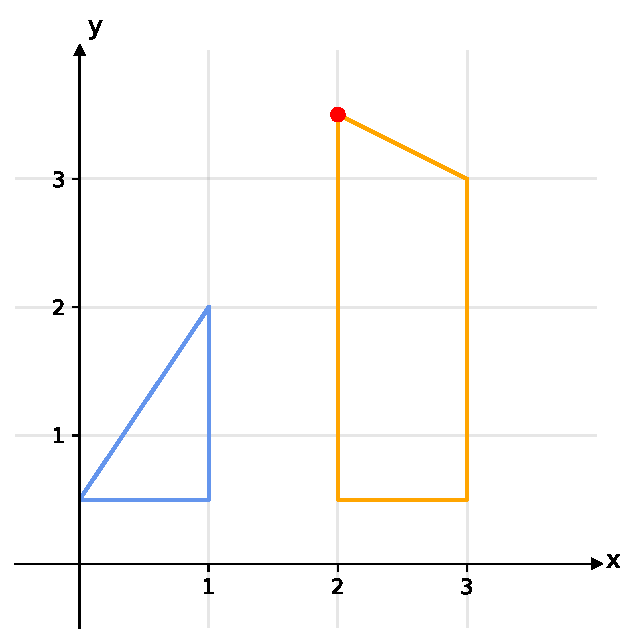
\includegraphics[width=0.6\textwidth]{Images/dp.pdf}
    \label{fig:dp}
    \subcaption{
        The set of feasible solutions is no longer convex and is the union of the polytope $P_1$ (blue line segments) and the polytope $P_2$ (orange line segments). The optimal solution $x^*$ is the point in the feasible region with the biggest $y$-value (red point).}
\end{figure}
\unsure{how to write problem in dp form?}

\subsubsection{Solving DPs}
A disjunctive model can be formulated as mixed-integer program and solved by corresponding techniques ( see \cref{Section:MIP}). Disjunctions can be expressed by linear constraints and integer variables by using the big-M method. Suppose we have a disjunction with $k$ terms:
\begin{equation*}
    (\bold a_1 \tran \bold x \leq b_1) \lor (\bold a_2 \tran \bold x \leq b_2) ... \lor (\bold a_k \tran \bold x \leq b_k)
\end{equation*}
We use the binary variable $z_i$ and enforce with the constraint $z_1 +  z_2 + ... + z_k$ that at least one of the $k$ terms is true. If $z_i=1$, term $(\bold a_i \tran \bold x \leq b_i)$ is enforced. See \cref{Section:MIP} on how to express indicator constraints with linear constraints and binary variables. Often the $M$ constant has to be large to be inactive if $z_i=0$. However, a large $M$ leads to a weaker LP relaxation which impacts the runtime of the Branch-and-Bound algorithm \cite{aps_mosek_nodate}. 

Another possibility is to convexify the feasible region and solve the resulting linear program. The idea is to build the convex hull of the union of polyhedral points in a higher dimension and project the solution back to the original dimension of the problem. \todo{more detail}


\subsection{Cutting Planes} \label{Section:cuts}
Let us consider an optimization problem with decision variables $\bold x$. A \textit{cutting plane} or \textit{cut} is an inequality that does not remove any feasible solution to the problem and is defined as: 
\begin{equation} \label{Eq:cuts}
    \sum_{i=1}^n \alpha_i x_i \leq \alpha_0
\end{equation} 
where $\alpha_i \in \mathbb{R}$. Usually, cutting planes are used to cut off solutions to the relaxed problem $\bold x^{LP}$ that are infeasible in the original problem. If there exists a hyperplane that separates $\bold x^{LP}$ from the actual feasible region, there usually exist multiple hyperplanes. As we want to tighten the search space, we are interested in cuts that remove cut off many infeasible points at once. There are different scores to estimate the quality of a cut. One scoring measure is \textit{efficacy} which is the distance from $\bold x^{LP}$ to the cutting plane:
\begin{equation}
    \text{eff}(\bold \alpha, \bold x^{LP}) := \frac{\boldsymbol \alpha \tran \bold x^{LP} - \alpha_0}{\lVert \boldsymbol \alpha \rVert}
\end{equation}

\cite{turner_adaptive_2023}

The cuts relevant for this thesis are explained in detail below. 
\todo{numerical issues, finding good cut can be expensive}
\todo[inline]{example + visualization}

\subsubsection{No-Good Cuts}
Given a mixed-integer problem as in \cref{problem:MIP} $\mathcal{P}$. If a solution to the relaxed LP $\bold x^{LP}$ is not a feasible solution to $\mathcal{P}$, we want to exclude the solution from the search space. The following \textit{no-good cut} is added to $\mathcal{P}$ and cuts off exactly $\bold x^{LP}$:
\begin{equation*}
    \sum_{j: x_j^{MP}=0} (1 - x_{j}) + \sum_{j: x_j^{MP}=1} x_j \quad \leq \quad n -1
\end{equation*}
where $n$ is the dimension of $\bold x^{LP}$. 

Such a cut usually tightens the feasible region of $\mathcal{P}$ marginally and it would require a large number of no-good cuts to arrive at the integer hull.

\subsubsection{Combinatorial Benders' Cuts}
Given a problem of the form:
\begin{mini!}
    {\scriptstyle \bold x, \bold z}{\bold c \tran \bold x}{}{} \label[problem]{problem:mathematical_program_CB}
    \addConstraint{\bold F \bold x \leq \bold g}
    \addConstraint{\bold D \bold z \leq \bold e}
    \addConstraint{x_j = 1 \implies \bold a_{i,*} \tran \bold z \leq b_i \quad \forall i \in I}
    \addConstraint{x_j \in \{ 0,1 \}}
    \addConstraint{y_i \in \mathbb{R}}
\end{mini!}
As the objective does not depend on $\bold z$ and as the decision variables $\bold x, \bold z$ are independent apart from the indicator constraints, we can split the problem into a \textit{master problem} (MP) and a \textit{subproblem} (SP). Constraint \cref{problem:mathematical_program_CB} (d) is modeled using the big-M method: $\bold A \tran \bold z \leq \bold b + M(\bold 1- \bold x)$.
\unsure{write M as matrix, vector or constant}
\begin{mini!}
    {\scriptstyle \bold x}{\bold c\tran \bold x}{\text{\textbf{MP:}} \label[problem]{problem:MP}}{}
    \addConstraint{\bold F \bold x \leq \bold g}    
    \addConstraint{\bold x \in \mathbb{R}^n}
    \addConstraint{x_j \in \{ 0,1 \}}
\end{mini!}
The master problem ignores the constraints on $\bold z$. The subproblem depends on a solution $\bold x^{MP}$ to the master problem. 

\begin{mini!}
    {\scriptstyle \bold z}{0}{\text{\textbf{SP:}} \label[problem]{problem:SP}}{}
    \addConstraint{\bold D \bold z \leq \bold e}
    \addConstraint{\bold a_{i,*} \tran \bold z \leq b_i + M_i(1- x_{j}^{MP}) \quad \forall i \in I}
\end{mini!}
If solution $\bold x^{MP}$ leads to a feasible subproblem, $\bold x^{MP}$ is an optimal solution to \cref{problem:mathematical_program_CB}. If the problem is infeasible, $\bold x^{MP}$ is not a feasible solution for the original problem. In that case we want to add a cut that removes $\bold x^{MP}$ from the search space. Suppose we have access to a \textit{minimal infeasible subset} (MIS) $C$ that is a set of constraints in the infeasible subproblem that lead to infeasibility: 
\begin{mini!}
    {\scriptstyle \bold z}{0}{}{}
    \addConstraint{\bold D \bold z \leq \bold e}
    \addConstraint{\bold a_{i,*} \tran \bold z \leq b_i + M_i(1- x_{j}^{MP}) \quad \forall i \in C}
\end{mini!}

The \textit{combinatorial Benders' cut} is then: 
\begin{equation*}
    \sum_{j \in C: x_j^{MP}=0} (1 - x_{j}) + \sum_{j \in C: x_j^{MP}=1} x_j \quad \leq \quad |C| -1
\end{equation*}

A minimal infeasible subset can be found by studying the dual problem of the infeasible subproblem. As the subproblem is a linear problem, strong duality holds and an infeasible primal problem implies an unbounded dual problem (see \cref{Section:Linear Programming}).

To derive the dual problem of \cref{problem:SP} we write constraints (b) and (c) as one constraint and stack the variables in the vector $\bold y$: $\bold{\tilde A} \bold y \leq \bold{\tilde b}$. The dual is then:
\begin{maxi!}
    {\scriptstyle \boldsymbol \lambda}{\bold{\tilde b} \tran \boldsymbol \lambda}{}{}
    \addConstraint{\bold{\tilde A} \tran \boldsymbol \lambda = \bold 0}
    \addConstraint{\boldsymbol \lambda \geq \bold 0}
\end{maxi!}
As $\boldsymbol \lambda$ is a feasible solution the dual problem, the dual problem has at least one feasible solution and is never infeasible. In the case where the dual is unbounded, there exist multiple feasible solutions. We are interested in a feasible solution with $\boldsymbol \lambda \neq \bold 0$ and therefore add the constraint $\bold{\tilde b} \tran \boldsymbol \lambda = \bold 1$. Now that the objective function is hidden in the constraints we can set a different objective function.
The linear program to find minimal infeasible subsets is then:
\begin{maxi!}
    {\scriptstyle \boldsymbol \lambda}{\sum_i w_i \lambda_i}{\label[problem]{problem:mis_lp}}{} 
    \addConstraint{\bold{\tilde A} \tran \boldsymbol \lambda = \bold 0}
    \addConstraint{\boldsymbol \lambda \geq \bold 0}
    \addConstraint{\bold{\tilde b} \tran \boldsymbol \lambda = \bold 1}
\end{maxi!}
where $w_i$ is the weight corresponding to the dual variable $\lambda_i$. The support of each solution at a vertex of the feasible region of \cref{problem:mis_lp}  defines a minimal infeasible subsystem. By changing the weights in the objective, several MISs can be obtained for one infeasible MP solution. \cite{codato_combinatorial_2006}


\subsubsection{Intersection Cuts} \label{Section:intersection_cuts}

Given a problem of the form:
\begin{mini}
    {\scriptstyle \bold x}{\bold c \tran \bold x}{}{} \label[problem]{problem:mathematical_program_S_P}
    \addConstraint{\bold x \in S \cap P}
\end{mini} 
where $\bold c \in \mathbb{R}^n$, $P$ is a polyhedron and $S \subset \mathbb{R}^n$ a closed set. In the LP relaxation of \cref{problem:mathematical_program_S_P} the constraint becomes $\bold x \in P$. However, the relaxation might not be a good approximation of the true feasible region. The polyhedral approximation 
can be tightened by adding intersection cuts. 
\cite{bienstock_outer_product_free_sets}

% \todo{should be closed otherwise optimum not bounded}
% Instead of solving an optimization problem directly, a relaxed version of the problem is solved. For instance, instead of solving an ILP, one would solve the LP without integrality constraints. 

Let $\bold{\tilde x}$ be an optimal solution to the LP relaxation that is infeasible in the original problem: $\bold x \notin S$. %To derive an intersection cut, the intersection between the conic relaxation around $\tilde x$ and an $S$-free set $C$ containing $\tilde x$ is required. \cite{musalem_intersection_cuts}
The \textit{conic relaxation} at vertex $\bold{\tilde x}$ is a cone with apex $\bolde{\tilde x}$ and the neighbouring edges are the extreme rays. For a given set $S$, the convex set $C$ is \textit{$S$-free} if: $S \cap \text{int}(C) = \emptyset$. \cite{bienstock_outer_product_free_sets} The hyperplane intersecting $C$ and the conic relaxation is the \textit{intersection cut} and when added to the problem will cut off $\bold{\tilde x}$. Due to convexity of the feasible region and given that the cutoff area lies in $C$, all feasible solutions remain in the resulting polytope\todo{not necessarily polytope}. \cite{musalem_intersection_cuts}
In order to generate deep cuts, the $S$-free set should be maximal. An $S$-free set $C$ is \textit{maximal} if $C \not \subset C'$ for any $S$-free set $C'$. \cite{bienstock_outer_product_free_sets}

A diagram for the following problem is shown in \cref{fig:intersection_cut}: 
\begin{equation} \label[problem]{problem:intersection_cut_example}
    \text{max} \{y \, : \, 0 \leq x \leq 3 , \, 0.5 \leq y \leq 4, \, y \leq 1.5 x + 0.5, \, y \leq -0.5 x + 4.5, \, x,y \in \mathbb{Z} \}
\end{equation}
The problem is a mixed-interger progam as it has a linear objective, linear constraints and integrality constraints on the decision variables $x,y$. The optimal solution of the relaxed linear program to \cref{problem:intersection_cut_example} is $\tilde x = (2,3.5)$\unsure{rename?, write as vector}. The set $S$ contains all integer points: $S = \mathbb{Z}$. A possible $S$-free set $C$ is a disk where the center is $\tilde x$ and the radius the distance $\lambda$ between $\tilde x$ and the closest integer, in our case $\lambda = 0.5$.  The conic relaxation is the cone with apex $\tilde x$ and the active constraints at $\tilde x$: $y \leq 1.5x + 0.5$ and $y \leq -0.5 x + 4.5$. \todo{verify correctness, ACTIVE CONSTRAINTS != EXTREME RAYS (n-D)} The intersection between the circle $C$ and the conic relaxation are the points $P_1 \approx (1.7,3.1)$ and $P_2 \approx (2.5,3.3)$. The area between $\tilde x$ and the line going through $P_1$ and $P_2$ is cutoff by adding a constraint to the relaxed LP of \cref{problem:intersection_cut_example}. \unsure{differentiate point from vector in notation?}

\begin{figure}[H]
    \caption{diagram of intersection cut for \cref{problem:intersection_cut_example}}
    \centering
    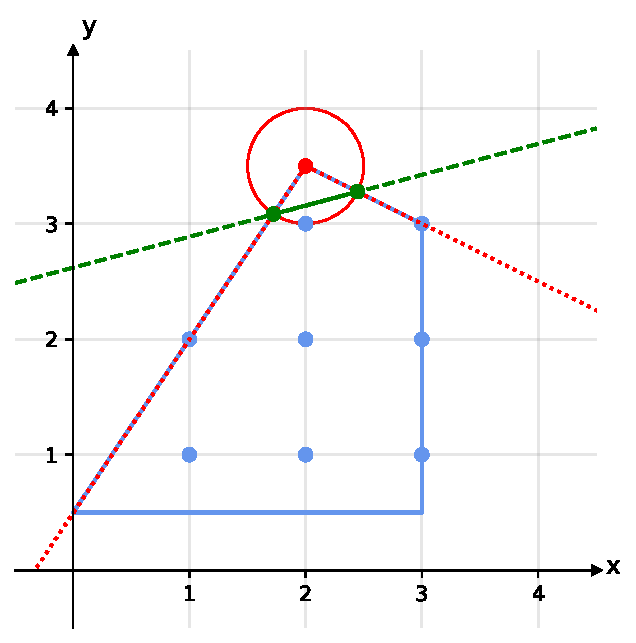
\includegraphics[width=0.6\textwidth]{Images/intersection_cut.pdf}
    \label{fig:intersection_cut}
    \subcaption{
        The feasible points of the MIP are the integer points respecting the polyhedral constraints (blue points). The set of feasible solutions to the relaxed LP is are all the points in the interior or on the boundary of the polytope (blue line segments). The optimal solution $\tilde x$ to the relaxed LP is the point in the feasible region with the biggest $y$-value (red point). A possible $S$-free set $C$ is a disk with center $\tilde x$ and the radius being the distance between $\tilde x$ and the closest integer (red circle). The conic relaxation are the extreme rays generated by $\tilde x$ which correspond to the two active constraints at $\tilde x$ (is indicated by the dotted, red line). The intersection of the conic relaxation and $C$ are the two points in green. The intersection cut is constructed with the line going through the intersecting points (dashed line in green). The area above the green line will be cut off and $\tilde x$ is no longer a feasible solution.}
\end{figure} \todo{update $\tilde x$}

The conic relaxation at $\tilde x$ is a pointed cone with extreme point $\tilde x$ and can be written as: 
\begin{equation} \label{Eq:conic_relaxation}
    P' = \{ \bold{\tilde x} + \sum_{j=1}^n \lambda_j \bold r^j : \boldsymbol \lambda \geq 0 \}
\end{equation}
or as:
\begin{equation} \label{Eq:conic_relaxation_polyhedral}
    P' = \{\bold x|\bold{\tilde Ax} \leq \bold{\tilde b}\}
\end{equation} \unsure{confusing to have two x?}
where $r^j$ are the extreme rays, $\bold{\tilde A}$ is an invertible $n\times n$ submatrix of $ \bold A$ such that the rows are linearly independent and are a basis for $\bold{\tilde x}$. 
% If the original problem is brought in the form $ \bold Ax \leq b$, the bounds on $x$ are included in $ \bold A$ and therefore $m \geq n$. 
A basis for $\bold{\tilde x}$ are the nonbasic constraints at $\bold{\tilde x}$.
If a constraint is nonbasic, the corresponding slack variable of the standard form is nonbasic and therefore 0. This implies that the constraint is active. 

After deriving the conic relaxation, we have $\bold{\tilde x} = \bold{\tilde A^{-1} \tilde b}$ and $\bold r^j= - \boldsymbol{\tilde A^{-1}_{*,j}}$. For each extreme ray $\bold r^j$ there either exists an intersection with the boundary of $C$ in which case $\lambda^*_j > 0$ is the step length or the extreme ray is contained in $C$ and $\lambda^*_j= \infty$. \unsure{power number in bold or not}

The \textit{intersection cut} is defined as:
\begin{equation} \label{Eq:interscetion_cut}
    \sum_{i=1}^n (\tilde a_{i,*}x - \tilde b_i)/ \lambda_i^* \leq -1
\end{equation}
If we reformulate \cref{problem:interscetion_cut} we see that it matches the definition in \cref{Eq:cuts}:
\begin{align}
    \sum_{i=1}^n (\tilde a_{i,*}x - \tilde b_i)/ \lambda_i^* &\leq -1 \\
    \sum_{i=1}^n ((1/ \lambda_i^*)\tilde a_{i,*}x - (1/ \lambda_i^*)\tilde b_i) &\leq -1 \\ 
    \sum_{i=1}^n (1/ \lambda_i^*)\tilde a_{i,*}x - \sum_{i=1}^n  (1/ \lambda_i^*)\tilde b_i &\leq -1 \\
    \sum_{i=1}^n (1/ \lambda_i^*)\tilde a_{i,*}x & \leq -1 + \sum_{i=1}^n  (1/ \lambda_i^*)\tilde b_i
\end{align}
\begin{equation*}
    \alpha_0 = -1 + \sum_{i=1}^n  (1/ \lambda_i^*)\tilde b_i \quad \quad \alpha_j = \sum_{i=1}^n (1/ \lambda_i^*)\tilde a_{i,j}x
\end{equation*} \todo{vectors in bold}

\cite{bienstock_outer_product_free_sets}

\todo[inline]{explain why x is cut off}
\todo[inline]{should -1 be eps?}
\unsure[inline]{does opt sense matter?}
% \todo[inline]{different cut formulations}
\todo[inline]{use bar or tilde in intersection cuts? tilde already used for combinatorial benders}
\todo[inline]{polyhedral P vs primal P vs optimization problem}